
\subsection{FPGA Simulation Results}
While testing \textit{ChaosM} with the aim of accomplishing FR3
some problems were encountered. These tests show post-route simulation on our
toplevel vhdl design. This includes the ebi controller, clock controller and the pipeline(s).
The tests looked like this:

\begin{itemize}
\item Load a program into the processors’ instruction memory. The program will load from its input buffer and store to its output buffer.\\
\item Load input into the first core’s input buffer. The data loaded was “BEEF” for the first pipeline and “1EEF” for the second pipeline (if applicable).\\
\item Read the result from the last core output buffer. The result can be read from the signal called “EBI data”.\\
\end{itemize}


\paragraph{First Test}
The first test was one pipeline with four cores. The timing simulation of this test is
 shown in diagram \ref{fig:one_pipe_four_core}. As the diagram shows,
 the simulation outputs the correct results shown by signal in orange at the point
 marked by the yellow, vertical line.

 \begin{figure}[H]
    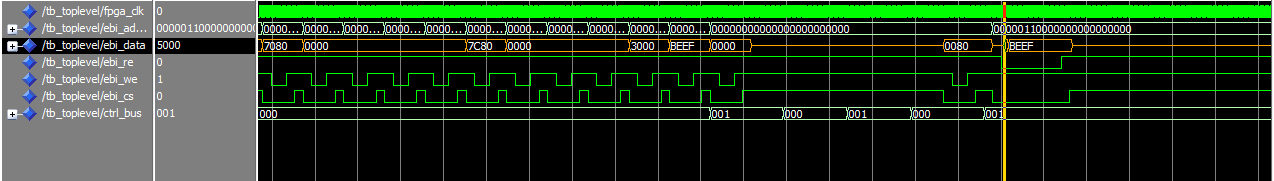
\includegraphics[width=1.3\textwidth]{figures/fpga/result_1_pipe_4_cores.PNG}
    \caption{Result from timing simulation of one pipeline with four cores.}
    \label{fig:one_pipe_four_core}
\end{figure}

\paragraph{Second Test}
The second test was two pipelines with four cores in each. The timing simulation
of this test did not work as expected. Out of the two pipelines simulated only one
gave correct results, see diagram \ref{fig:two_pipe_four_core}. The first core
outputted only zeros, as the yellow line shows,  while the second pipeline outputted the correct result “1EEF”.

\begin{figure}[H]
    \centering
    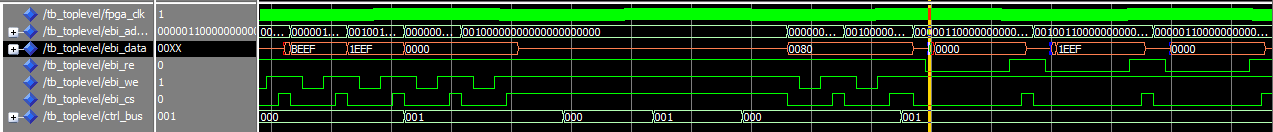
\includegraphics[width=1.3\textwidth]{figures/fpga/result_2_pipe_4_cores.PNG}
    \caption{Result from timing simulation of two pipelines with four cores each.}
    \label{fig:two_pipe_four_core}
\end{figure}


\subsection{FPGA Configuration Results}
Even though one pipeline with four cores simulated correctly in ModelSim, the configured FPGA
did not work as in the simulation. It behaved nondeterministically with little to no pattern
in the outputted results. A lot of debugging was done and it seems as though the problems
lie in the communication between the microcontroller and the FPGA.

